\section{测定硝酸钾在水里的溶解度并绘制它的溶解度曲线图\footnotemark}\label{sec:xssy-xzsy1}
\footnotetext{本实验编入了两种方法——溶质质量法和结晶析出法,教师可根据实际情况任选一种。
    选用溶质质量法时,可让每个实验小组分别测定一个温度下的溶解度,然后综合全班各组测出的数据,绘出溶解度曲线图。
    选用结晶析出法时,可让每个实验小组测两个温度下的溶解度。
}

\begin{shiyanmudi}
    1. 学会测定固体物质的溶解度,加深对溶解度概念的理解; 2. 学会溶解度曲线图的绘制方法; 3. 学会使用温度计和水浴加热的操作技能。
\end{shiyanmudi}


\begin{shiyanyongpin}
    托盘天平、烧杯(250 毫升)、试管、玻璃棒、温度计、酒精灯、量筒(10 毫升)、铁架台(带铁圈和铁夹)、蒸发皿、石棉网、干燥器、坩埚钳。

    硝酸钾、蒸馏水。
\end{shiyanyongpin}


\subsection{溶质质量法}


\begin{shiyanbuzhou}
    \begin{wrapfigure}[16]{r}{5cm}
        \centering
        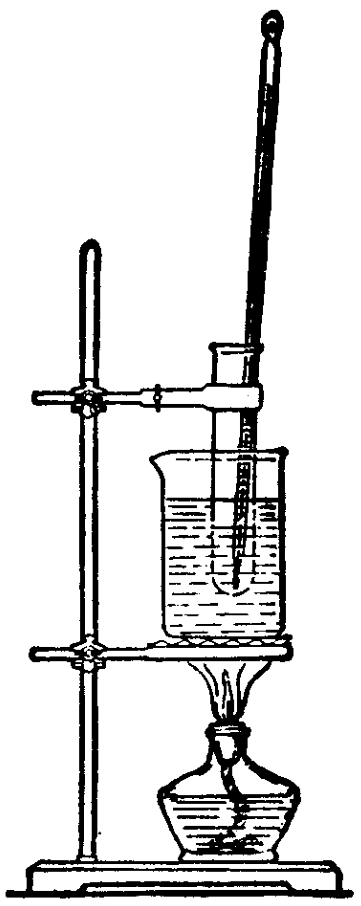
\includegraphics[width=3.5cm]{../pic/czhx1-xssy-28}
        \caption{测定溶解度}\label{fig:xssy-28}
    \end{wrapfigure}

    1. 用天平称量一个干燥的蒸发皿的质量,并将称量的数值记入下面的表里。

    2. 用量筒量取 10 毫升蒸馏水,倒入试管里。然后把一支温度计放在试管里(如图 \ref{fig:xssy-28} 所示 )。
    在烧杯里倒入约 150 毫升水,将试管(连水带温度计)放入烧杯里,进行水浴%
    \footnote{当被加热物质要求受热均匀时,而温度不能超过 100 ℃时,可利用水浴。}加热。
    利用酒精灯控制水温,使试管里温度保持相对稳定。\footnote{如果欲测温度是 20 ℃, 那么在 18 ~ 22 ℃ 时保持稳定也可以。}

    保持恒温后,逐渐向试管里加入少量硝酸钾的晶体,用玻璃棒搅拌,直到在五分钟内不再溶解为止。

    3. 取下试管,把里面的硝酸钾溶液倾倒在已称量过的蒸发皿里(注意不要把未溶解的硝酸钾晶体倒入)。
    然后称量,把数值记入下表里。

    4. 把蒸发皿放到酒精灯上加热,边加热边搅拌。待析出晶体较多时,改用微火加热,直到水分完全蒸发掉为止。
    待稍冷后,把蒸发皿放入干燥器中冷却,冷却后,称量,直到两次称量的质量结果相差不超过 $0.1$ 克。把数据记入下表中。

    5. 利用所测数据,根据下式计算出硝酸钾在指定的一个温度下的溶解度 $S$。

    \begin{tblr}{
        hlines, vlines,
        columns={c,m, 5em},
        column{1}={3em},
    }
        {温度\\[-.3em]℃}
            & {蒸发皿\\[-.5em]的质量\\[-.5em]$a$(克)}
            & {(蒸发皿\\[-.5em] $+$ 溶液)\\[-.5em]的质量\\[-.5em] $b$(克)}
            & {(蒸发皿\\[-.5em] $+$ 晶体)\\[-.5em]的质量\\[-.5em] $c$(克)}
            & {水的质量\\[-.5em] $b - c$(克)}
            & {晶体的质量\\[-.5em] $c - a$(克)}
            & {溶解度\\[-.5em] $S$(克)} \\
        \\
        \\
        \\
        \\
        \\
    \end{tblr}

    \jiange
    $$ \text{溶解度(克)} \; S = \dfrac{100(c - a)}{b - c} $$

    把本组和其它各组在不同温度下测定的数据分别填入上表里。
    欲测温度可分别选择为 10 ℃、20 ℃、30 ℃、40 ℃、50 ℃等。

    6. 根据所得到的数据,以温度为横坐标、溶解度为纵坐标,绘制溶解度曲线图。
\end{shiyanbuzhou}


\begin{wentihetaolun}
    1. 用水浴加热时,为什么一定要把试管内的液体全部浸没在水浴里?

    2. 测定硝酸钾的溶解度时,试管里除温度应保持恒定外,还应留有一些未溶解的硝酸钾,为什么?

    3. 为什么倾倒出来的饱和溶液里不能混有固体?

    4. 把你测得的溶解度跟课本中的溶解度数据进行比较,并作简单的分析。通过本实验,你有什么经验教训和体会?
\end{wentihetaolun}


\subsection{结晶析出法}

\begin{shiyanbuzhou}
    1. 在托盘天平上分别称量硝酸钾 2.5 克、3.5 克、5.0 克、7.0 克、9.0 克,
    然后依次放入已经编好号的干燥的试管里。注意不要把硝酸钾粘在试管壁上。

    2. 用量筒量取 10 毫升蒸馏水。在五个试管里分别加入 10 毫升蒸馏水。

    3. 在每个试管里插入一根玻璃棒,然后依次把每个试管放在水浴里进行加热,
    边加热边搅拌,使硝酸钾固体全部溶解。在加热过程中,要用温度计测水温。
    注意不要使温度上升过高,以致下一步结晶析出需要的时间太长\footnote{
        可以进行粗略计算。例如,20 ℃ 时硝钾溶解度为 31.6 克,那么 20 ℃ 时在 10 毫升水里最多能溶解 3.16 克硝酸钾。
        2 号试管中有 3.5 克硝酸钾,大约在略高于 20 ℃ 时能全部溶解,因此加热温度不要高于 30 ℃,以此类推。
    }。

    4. 当硝酸钾全部溶解后,可把试管拿出水面,插入一根干净的温度计,
    一边用玻璃棒轻轻地摩擦管壁,一边观察温度计的读数。
    这时一定要耐心和细心,当有晶体析出时,立即读取温度,并作记录。

    5. 把试管再放入水浴里加热,使硝酸钾溶解。然后重复上面的操作,再测定晶体析出时的温度。
    对比两次的读数,如果差别较大,再重复测定一次。

    6. 根据所测数据,计算硝酸钾的溶解度。

    \begin{tblr}{
        hlines, vlines,
        columns={c},
        column{4-6}={3em},
    }
        \SetCell[r=2]{m} 编号
            & {\SetCell[r=2]{m} 硝酸钾的质量\\(克)}
            & \SetCell[r=2]{m} {水的体积\\(毫升)}
            & \SetCell[c=3]{c} 结晶析出的温度(℃) & &
            & \SetCell[r=2]{m} {溶解度\\(克)} \\
        & & & 1 & 2 & 平均值 & \\
        1 & 2.5 & 10 & & & & \\
        2 & 3.5 & 10 & & & & \\
        3 & 5.0 & 10 & & & & \\
        4 & 7.0 & 10 & & & & \\
        5 & 9.0 & 10 & & & & \\
    \end{tblr}


    \jiange
    7. 根据所得到的数据,以温度为横坐标、溶解度为纵坐标,绘制溶解度曲线图。
\end{shiyanbuzhou}


\begin{wentihetaolun}
    把你测得的溶解度跟课本中的溶解度数据进行比较,并作简单的分析。通过本实验,你有什么经验教训和体会?
\end{wentihetaolun}


